% https://www.overleaf.com/read/jydxqkkkskzp
% https://github.com/MCG-NKU/NSFC-LaTex
% by Ming-Ming Cheng https://mmcheng.net

%\documentclass[12pt]{article}
\documentclass[12pt,AutoFakeBold]{article}
\usepackage[UTF8]{ctex}
\usepackage{nsfc}
\usepackage{enumitem}

\newcommand{\cmm}[1]{\textcolor[rgb]{0,0.6,0}{CMM: #1}}
\newcommand{\todo}[1]{{\textcolor{red}{\bf [#1]}}}
\newcommand{\myPara}[1]{\paragraph{#1:}}

% yaxing: begin
\usepackage[resetlabels]{multibib}
\newcites{sec}{Reference}
\usepackage{color}

\newcommand{\upcite}[1]{{\textsuperscript{\cite{#1}}}}
\newcommand{\sprod}[2]{\left\langle #1,#2 \right\rangle}
\newcommand{\minisection}[1]{\vspace{0.04in}\noindent {\bf #1}\ \ }


%  \iffalse
\newcommand{\revision}[1]{{\color{blue} #1}}
\graphicspath{{figures/}}


\begin{document}

\begin{figure}[h]
    \centering
    
\includegraphics[width=.7\linewidth]{figures/logo.jpeg}
\end{figure}

\vspace{1cm}
\hrulefill
    \begin{center}
        \Huge\textbf{《人工智能导论》探究报告\\ 图像超分\textcolor{red}{为例} }
     
    \end{center}   

\hrulefill
\vspace{1cm}

\begin{table}[h]
    \centering
    \large
    \begin{tabular}{ll}
    \textbf{姓名:XXX   \quad  学号:0000000} \quad SRCNN  \\
    \textbf{姓名:XXX    \quad  学号:0000000} \quad VDSR \\
    \textbf{姓名:XXX    \quad  学号:0000000} \quad SRGAN \\
    \end{tabular}
\end{table}

\newpage

%%%%%%%%% TITLE

\title{\kaishu 作业正文}

\maketitle




\section{问题描述(\revision{文字描述与形式化定义,组员共同完成})}


\section{核心内容(\revision{三篇论文三位组员分别负责,拓展阅读论文组员共同选题和完成,描述论文动机,方法,实验结果等关键内容}):}

\subsection{规定论文题目1}
\subsubsection{论文动机}

如何使用插入图像:


\begin{figure*}[h]
    \centering
    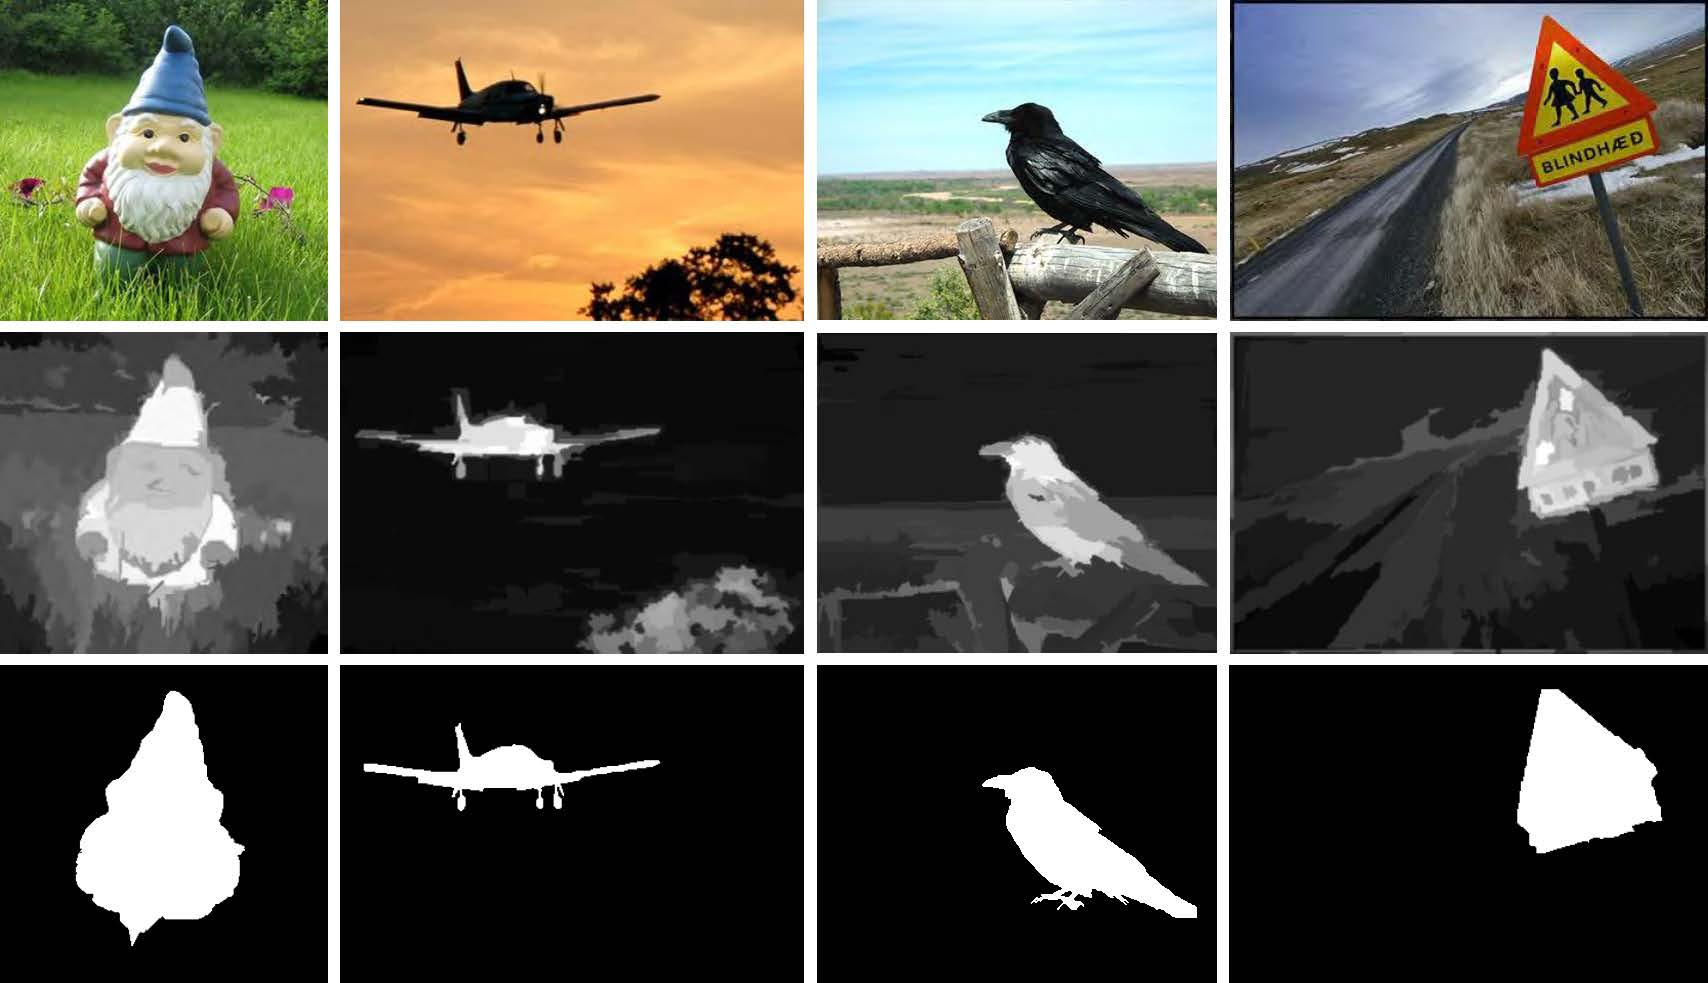
\includegraphics[width=1\linewidth]{figures/teaser.jpg}  
    %\vspace{-6mm}
    \caption{\small 示意图}
    \label{fig:framework}
    %\vspace{-15pt}
\end{figure*}



\subsubsection{方法}

如何使用公式:

\vspace{-3pt}
\begin{equation}
 \mathcal{L}_{kdl}^{e}= \sum _{l} \gamma_{l} \left \| D_{T}(\mathbf{x_{t}^{1}})_{l} -  E_{S}(\mathbf{x_{t}^{1}} )_{l}  \right \|_{1}
\label{eq:kdl_e}
\end{equation} 

\subsubsection{实验结果}

如何插入表格:

\begin{table}[h]
  \centering
  \begin{tabular}{@{}lc@{}}
    \hline    \hline

    Method & Frobnability \\
    \hline
    Theirs & Frumpy \\
        \hline

    Yours & Frobbly \\
        \hline

    Ours & Makes one's heart Frob\\
    \hline    \hline

  \end{tabular}
  \caption{Results.   Ours is better.}
  \label{tab:example}
\end{table}
\subsection{规定论文题目2}

\subsection{规定论文题目3}

\subsection{自选论文题目 (\revision{组员共同完成})}




\section{思考与理解(\revision{联系与区别、尚未解决的问题、未来研究趋势等,组员共同完成}):}

\subsection{联系与区别}

\subsection{尚未解决的问题}


\subsection{未来研究趋势}

如何添加参考文献:

图像到图像转换基本思想是将给定源域图像映射到目标域,在此过程中输出图像具有两个特点:(1)保持输入图像结构、姿势信息;(2)获取目标域图像风格、属性、外表特征。图像到图像转换最早追溯到图像类比\upcite{hertzmann2001image}开始, Hertzmann等人\upcite{efros1999texture}提出单个输入-输出训练图像对的非参数纹理模型。 最近的方法\upcite{long2015fully}使用输入输出示例的数据集来学习使用卷积神经网络(CNN)的参数翻译函数。针对输出为RGB的图像到图像转换,近年来相关研究主要集中于基于生成对抗网络(GAN)的学习方法,其从数据要求角度通常分为二类:监督方式图像到图像转换和非监督方式图像到图像转换。监督方式图像到图像转换中,Phillip等人\upcite{pix2pix2017}基于U-Net构建一种包含编码器-解码器的生成器架构:Pix2pix,中科院团队\upcite{song2018geometry}在图像转换中引入关键点信息



{\small
\bibliography{longstrings,Cmm}
\bibliographystyle{unsrt}
}

\end{document}
